\section{Введение}

    Наверное, что-то про модель Хасселя надо сказать.

    Популяционная модель Хасселя.

    Этого мало.

\section{Что-то после введения}

    Математическая запись модели:

    \[x_{t+1} = \frac{\alpha x_t^2}{(\beta + x_t)^6}\]

    где \(\alpha, \beta\) - параметры. Зафиксируем параметр \(\alpha = 1\). Параметр \(\beta\) изменяется в диапазоне \([0; 0.6]\)    

    \begin{equation}
        \label{eq1}
        x = \frac{\alpha x^2}{(\beta + x)^6}
    \end{equation}
    
    \[1 = \frac{\alpha x}{(\beta + x)^6}\]

    \[\alpha x = (\beta + x)^6\]

    Аналитически это уравнение не решается. Для нахождения корней будем использовать метод Ньютона.

    В зависимости от конкретных значений параметра \(\beta\) данное уравнение может иметь от одного до трех корней.
    
    *графики какие-нибудь*

    Для того, чтобы найти корни с помощью метода Ньютона рассмотрим уравнение 
    
    \[x - \frac{\alpha x^2}{(\beta + x)^6} = 0\]

    При \(\beta \approx 0.582355932\) уравнение имеет два корня: \(x_0 = 0\) и \(\bar{x}_1 \approx 0.116471186636\). При \(\beta < 0.582355932\) - три корня,а при \(\beta > 0.582355932\) - один корень \(x_0 = 0\).
    
    Корень == точке равновесия.

    Можно построить временные ряды.

    \begin{figure*}[h]
        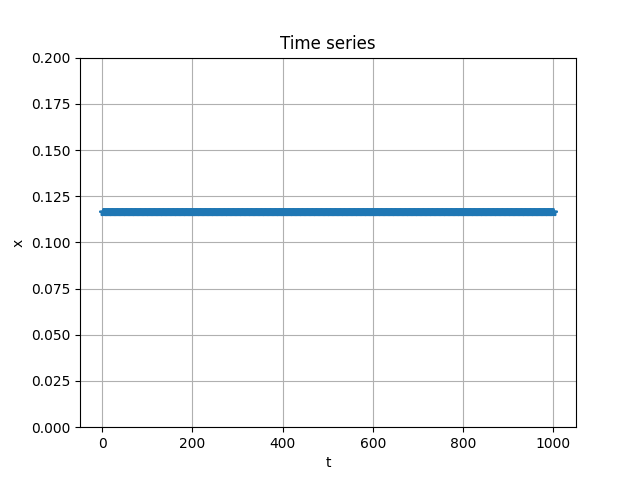
\includegraphics[scale=0.8]{images/Time_series_x_011647_b_0582355932.png}    
        \caption{Временной ряд при \(x_0 \approx 0.11647\) и \(\beta \approx 0.582355932\)}
    \end{figure*}

    Наверное, еще какие-нибудь ряды надо вставить\dots Только что надо показать на них?

\section{Итоги}

    Итак, что-то сделано.

    На что можно ссылаться?

    Для построения графиков использовались Python 3.9, mathplotlib, GeoGebra. Для нахождения корней методом Ньютона --- Python 3.9, GeoGebra.
